\newpage
\section*{Appendix}
\subsection*{MLP Binary Connect Architecture}
\begin{table}[H]
\begin{center}
\begin{tabular}{  c  }
\hline
   Dropout p = 0.2 \\ 
   Fully Connected Layer (units = 2048, bias = False) \\
   ReLU \\
   Batch Normalization Layer (gain = 1, bias = 0)  \\ \hline
   Dropout p = 0.2 \\ 
   Fully Connected Layer (units = 2048, bias = False)  \\
   ReLU  \\
   Batch Normalization Layer (gain = 1, bias = 0) \\ \hline
   Dropout p = 0.2 \\ 
   Fully Connected Layer (units = 2048, bias = False) \\
   ReLU  \\
   Batch Normalization Layer (gain = 1, bias = 0) \\ \hline
   Dropout p = 0.2 \\ 
   Fully Connected Layer (units = 2048, bias = False)  \\
   Batch Normalization Layer (gain = 1, bias = 0)  \\ 
   Softmax  \\\hline
    % \caption{MLP Binary Connect Architechture}
\end{tabular}
% \caption{\label{tab:7.1} Mean square error loss of Snelson dataset for different temperature.}
\end{center}
\end{table}

\subsection*{VGG Binary Connect Architecture}
\begin{table}[H]
\begin{center}
\begin{tabular}{ c }
\hline
   Convolutional Layer (channels = 128, kernel-size = 3×3, bias = False, padding = same)\\ 
   ReLU \\
   Batch Normalization Layer (gain = 1, bias = 0)  \\
   Convolutional Layer (channels = 128, kernel-size = 3×3, bias = False, padding = same) \\ 
   ReLU \\
   Max Pooling Layer (size = 2×2, stride = 2×2)  \\
   Batch Normalization Layer (gain = 1, bias = 0) \\ \hline
   Convolutional Layer (channels = 256, kernel-size = 3×3, bias = False, padding = same)\\ 
   ReLU \\
   Batch Normalization Layer (gain = 1, bias = 0)  \\
   Convolutional Layer (channels = 256, kernel-size = 3×3, bias = False, padding = same) \\ 
   ReLU \\
   Max Pooling Layer (size = 2×2, stride = 2×2)  \\
   Batch Normalization Layer (gain = 1, bias = 0)  \\ \hline
   Convolutional Layer (channels = 512, kernel-size = 3×3, bias = False, padding = same) \\ 
   ReLU  \\
   Batch Normalization Layer (gain = 1, bias = 0) \\
   Convolutional Layer (channels = 512, kernel-size = 3×3, bias = False, padding = same) \\ 
   ReLU \\
   Max Pooling Layer (size = 2×2, stride = 2×2) \\
   Batch Normalization Layer (gain = 1, bias = 0)  \\ \hline
   Fully Connected Layer (units = 1024, bias = False) \\      
   ReLU \\      
   Batch Normalization Layer (gain = 1, bias = 0)  \\ \hline
   Fully Connected Layer (units = 1024, bias = False) \\      
   ReLU \\      
   Batch Normalization Layer (gain = 1, bias = 0) \\ \hline
   Fully Connected Layer (units = 10, bias = False)  \\      
   Batch Normalization Layer (gain = 1, bias = 0) \\
   Softmax \\ \hline
\end{tabular}
% \caption{\label{tab:7.2} Mean square error loss of Snelson dataset for different temperature.}
\end{center}
\end{table}


\subsection*{MLP Binary Connect Architecture for Continual Learning}

\begin{table}[H]
\begin{center}
\begin{tabular}{  c  }
\hline
   Fully Connected Layer (units = 100, bias = False) \\
   ReLU  \\
   Batch Normalization Layer (gain = 1, bias = 0) \\ \hline
   Fully Connected Layer (units = 100, bias = False)  \\
   ReLU  \\
   Batch Normalization Layer (gain = 1, bias = 0) \\ \hline
   Fully Connected Layer (units = 100, bias = False)   \\
   ReLU \\
   Batch Normalization Layer (gain = 1, bias = 0)  \\ 
   Softmax \\\hline
\end{tabular}
% \caption{\label{tab:7.3} Mean square error loss of Snelson dataset for different temperature.}
\end{center}
\end{table}


\subsection*{LRNet Architecture (MNIST)}

\begin{table}[H]
\begin{center}
\begin{tabular}{  c  }
\hline
   Convolutional Layer (channels = 32, kernel-size = 5×5, bias = False, padding = same)\\ 
   Max Pooling Layer (size = 2×2, stride = 2×2)   \\
   Batch Normalization Layer (gain = 1, bias = 0) \\ 
   ReLU  \\ \hline

   Convolutional Layer (channels = 64, kernel-size = 5×5, bias = False, padding = same) \\ 
   Max Pooling Layer (size = 2×2, stride = 2×2) \\
   Batch Normalization Layer (gain = 1, bias = 0) \\ 
   ReLU \\ \hline   
   
   Fully Connected Layer (units = 512, bias = False) \\
   Batch Normalization Layer (gain = 1, bias = 0) \\ 
   ReLU \\ \hline
   
   Fully Connected Layer (units = 10, bias = False)  \\
   Batch Normalization Layer (gain = 1, bias = 0) \\ 
   Softmax   \\\hline

\end{tabular}
% \caption{\label{tab:7.4} Mean square error loss of Snelson dataset for different temperature.}
\end{center}
\end{table}


\subsection*{LRNet Architecture (CIFAR-10)}

\begin{table}[H]
\begin{center}
\begin{tabular}{  c  }
\hline
   Convolutional Layer (channels = 128, kernel-size = 3×3, bias = False, padding = same) \\ 
   Batch Normalization Layer (gain = 1, bias = 0) \\ 
   ReLU \\ \hline

   Convolutional Layer (channels = 128, kernel-size = 3×3, bias = False, padding = same)  \\ 
   Batch Normalization Layer (gain = 1, bias = 0)  \\
   Max Pooling Layer (size = 2×2, stride = 2×2)  \\
   ReLU \\ \hline

   Convolutional Layer (channels = 256, kernel-size = 3×3, bias = False, padding = same)\\ 
   Batch Normalization Layer (gain = 1, bias = 0) \\ 
   ReLU \\ \hline

   Convolutional Layer (channels = 256, kernel-size = 3×3, bias = False, padding = same) \\ 
   Batch Normalization Layer (gain = 1, bias = 0) \\
   Max Pooling Layer (size = 2×2, stride = 2×2)  \\
   ReLU  \\ \hline

   Convolutional Layer (channels = 512, kernel-size = 3×3, bias = False, padding = same) \\ 
   Batch Normalization Layer (gain = 1, bias = 0) \\ 
   ReLU \\ \hline
   
   Convolutional Layer (channels = 512, kernel-size = 3×3, bias = False, padding = same) \\ 
   Batch Normalization Layer (gain = 1, bias = 0) \\
   Max Pooling Layer (size = 2×2, stride = 2×2)  \\
   ReLU \\ \hline

   Fully Connected Layer (units = 1024, bias = False) \\
   Batch Normalization Layer (gain = 1, bias = 0)  \\ 
   ReLU  \\ \hline

   Fully Connected Layer (units = 10, bias = False)  \\
   Batch Normalization Layer (gain = 1, bias = 0) \\ 
   Softmax   \\\hline

\end{tabular}
% \caption{\label{tab:7.5} Mean square error loss of Snelson dataset for different temperature.}
\end{center}
\end{table}

\subsection*{Semantic Segmentation using BayesBiNN with augmented dataset}

 We generated 1260 images from 30 original images using the rotation, random horizontal flip, random vertical flip operations. The result for BayesBiNN with this extended dataset was still very poor and inconsistent with the other methods (STE and Full Precision). The results presented in Section 5.4 were to show the extent of difficulty to train BayesBiNN for segmentation task as even with such a small dataset and large number of epochs, it was still not even able to overfit. Following are some of the images obtained by using BayesBiNN with this bigger dataset:
 
 \begin{figure}[H]
     \centering
     \begin{subfigure}[b]{0.3\textwidth}
         \centering
         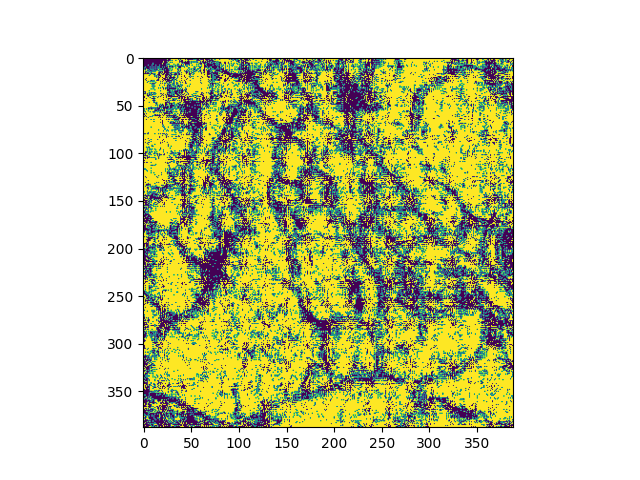
\includegraphics[width=1.4\textwidth]{../openreview/figs/output_43.png}
         \caption{Mask example 1}
     \end{subfigure}
     \hfill
     \begin{subfigure}[b]{0.3\textwidth}
         \centering
         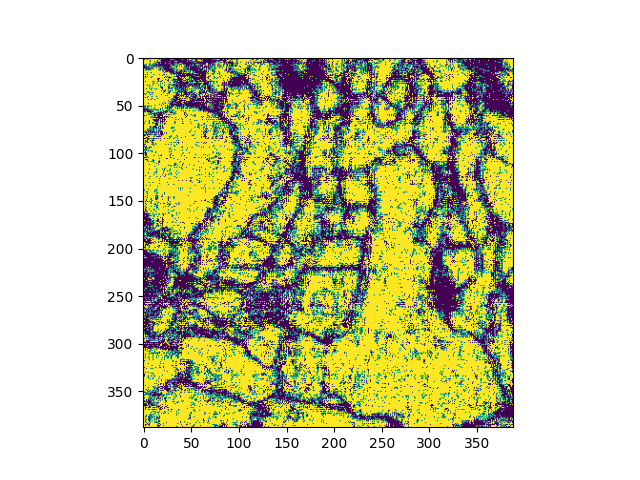
\includegraphics[width=1.4\textwidth]{../openreview/figs/output_27.png}
         \caption{Mask example 2}
     \end{subfigure}
     \hfill
\end{figure}